% Created by tikzDevice version 0.10.1 on 2017-12-03 20:41:14
% !TEX encoding = UTF-8 Unicode
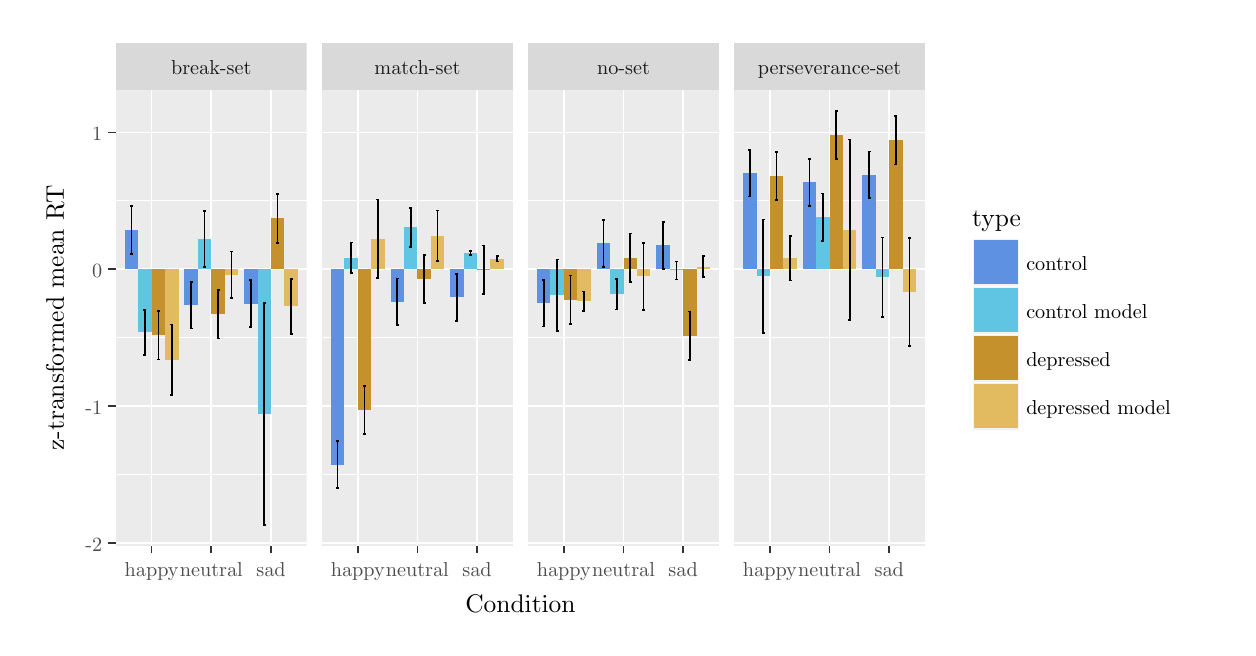
\begin{tikzpicture}[x=1pt,y=1pt]
\definecolor{fillColor}{RGB}{255,255,255}
\path[use as bounding box,fill=fillColor,fill opacity=0.00] (0,0) rectangle (433.62,216.81);
\begin{scope}
\path[clip] (  0.00,  0.00) rectangle (433.62,216.81);
\definecolor{drawColor}{RGB}{255,255,255}
\definecolor{fillColor}{RGB}{255,255,255}

\path[draw=drawColor,line width= 0.6pt,line join=round,line cap=round,fill=fillColor] (  0.00,  0.00) rectangle (433.62,216.81);
\end{scope}
\begin{scope}
\path[clip] ( 31.87, 29.59) rectangle (100.84,194.25);
\definecolor{fillColor}{gray}{0.92}

\path[fill=fillColor] ( 31.87, 29.59) rectangle (100.84,194.25);
\definecolor{drawColor}{RGB}{255,255,255}

\path[draw=drawColor,line width= 0.3pt,line join=round] ( 31.87, 55.41) --
	(100.84, 55.41);

\path[draw=drawColor,line width= 0.3pt,line join=round] ( 31.87,104.82) --
	(100.84,104.82);

\path[draw=drawColor,line width= 0.3pt,line join=round] ( 31.87,154.24) --
	(100.84,154.24);

\path[draw=drawColor,line width= 0.6pt,line join=round] ( 31.87, 30.71) --
	(100.84, 30.71);

\path[draw=drawColor,line width= 0.6pt,line join=round] ( 31.87, 80.12) --
	(100.84, 80.12);

\path[draw=drawColor,line width= 0.6pt,line join=round] ( 31.87,129.53) --
	(100.84,129.53);

\path[draw=drawColor,line width= 0.6pt,line join=round] ( 31.87,178.94) --
	(100.84,178.94);

\path[draw=drawColor,line width= 0.6pt,line join=round] ( 44.80, 29.59) --
	( 44.80,194.25);

\path[draw=drawColor,line width= 0.6pt,line join=round] ( 66.36, 29.59) --
	( 66.36,194.25);

\path[draw=drawColor,line width= 0.6pt,line join=round] ( 87.91, 29.59) --
	( 87.91,194.25);
\definecolor{fillColor}{RGB}{226,186,95}

\path[fill=fillColor] ( 49.65, 96.80) rectangle ( 54.50,129.53);
\definecolor{fillColor}{RGB}{196,145,45}

\path[fill=fillColor] ( 44.80,105.70) rectangle ( 49.65,129.53);
\definecolor{fillColor}{RGB}{95,197,226}

\path[fill=fillColor] ( 39.95,106.69) rectangle ( 44.80,129.53);
\definecolor{fillColor}{RGB}{95,145,226}

\path[fill=fillColor] ( 35.10,129.53) rectangle ( 39.95,143.71);
\definecolor{fillColor}{RGB}{226,186,95}

\path[fill=fillColor] ( 71.21,127.53) rectangle ( 76.06,129.53);
\definecolor{fillColor}{RGB}{196,145,45}

\path[fill=fillColor] ( 66.36,113.22) rectangle ( 71.21,129.53);
\definecolor{fillColor}{RGB}{95,197,226}

\path[fill=fillColor] ( 61.51,129.53) rectangle ( 66.36,140.39);
\definecolor{fillColor}{RGB}{95,145,226}

\path[fill=fillColor] ( 56.66,116.52) rectangle ( 61.51,129.53);
\definecolor{fillColor}{RGB}{226,186,95}

\path[fill=fillColor] ( 92.76,116.08) rectangle ( 97.61,129.53);
\definecolor{fillColor}{RGB}{196,145,45}

\path[fill=fillColor] ( 87.91,129.53) rectangle ( 92.76,147.86);
\definecolor{fillColor}{RGB}{95,197,226}

\path[fill=fillColor] ( 83.06, 77.25) rectangle ( 87.91,129.53);
\definecolor{fillColor}{RGB}{95,145,226}

\path[fill=fillColor] ( 78.21,117.09) rectangle ( 83.06,129.53);
\definecolor{drawColor}{RGB}{0,0,0}

\path[draw=drawColor,line width= 0.6pt,line join=round] ( 51.54,109.58) --
	( 52.62,109.58);

\path[draw=drawColor,line width= 0.6pt,line join=round] ( 52.08,109.58) --
	( 52.08, 84.02);

\path[draw=drawColor,line width= 0.6pt,line join=round] ( 51.54, 84.02) --
	( 52.62, 84.02);

\path[draw=drawColor,line width= 0.6pt,line join=round] ( 46.69,114.48) --
	( 47.77,114.48);

\path[draw=drawColor,line width= 0.6pt,line join=round] ( 47.23,114.48) --
	( 47.23, 96.93);

\path[draw=drawColor,line width= 0.6pt,line join=round] ( 46.69, 96.93) --
	( 47.77, 96.93);

\path[draw=drawColor,line width= 0.6pt,line join=round] ( 41.84,114.88) --
	( 42.92,114.88);

\path[draw=drawColor,line width= 0.6pt,line join=round] ( 42.38,114.88) --
	( 42.38, 98.50);

\path[draw=drawColor,line width= 0.6pt,line join=round] ( 41.84, 98.50) --
	( 42.92, 98.50);

\path[draw=drawColor,line width= 0.6pt,line join=round] ( 36.99,152.37) --
	( 38.07,152.37);

\path[draw=drawColor,line width= 0.6pt,line join=round] ( 37.53,152.37) --
	( 37.53,135.05);

\path[draw=drawColor,line width= 0.6pt,line join=round] ( 36.99,135.05) --
	( 38.07,135.05);

\path[draw=drawColor,line width= 0.6pt,line join=round] ( 73.09,135.89) --
	( 74.17,135.89);

\path[draw=drawColor,line width= 0.6pt,line join=round] ( 73.63,135.89) --
	( 73.63,119.17);

\path[draw=drawColor,line width= 0.6pt,line join=round] ( 73.09,119.17) --
	( 74.17,119.17);

\path[draw=drawColor,line width= 0.6pt,line join=round] ( 68.24,121.96) --
	( 69.32,121.96);

\path[draw=drawColor,line width= 0.6pt,line join=round] ( 68.78,121.96) --
	( 68.78,104.47);

\path[draw=drawColor,line width= 0.6pt,line join=round] ( 68.24,104.47) --
	( 69.32,104.47);

\path[draw=drawColor,line width= 0.6pt,line join=round] ( 63.39,150.45) --
	( 64.47,150.45);

\path[draw=drawColor,line width= 0.6pt,line join=round] ( 63.93,150.45) --
	( 63.93,130.33);

\path[draw=drawColor,line width= 0.6pt,line join=round] ( 63.39,130.33) --
	( 64.47,130.33);

\path[draw=drawColor,line width= 0.6pt,line join=round] ( 58.54,124.96) --
	( 59.62,124.96);

\path[draw=drawColor,line width= 0.6pt,line join=round] ( 59.08,124.96) --
	( 59.08,108.09);

\path[draw=drawColor,line width= 0.6pt,line join=round] ( 58.54,108.09) --
	( 59.62,108.09);

\path[draw=drawColor,line width= 0.6pt,line join=round] ( 94.65,126.06) --
	( 95.72,126.06);

\path[draw=drawColor,line width= 0.6pt,line join=round] ( 95.18,126.06) --
	( 95.18,106.09);

\path[draw=drawColor,line width= 0.6pt,line join=round] ( 94.65,106.09) --
	( 95.72,106.09);

\path[draw=drawColor,line width= 0.6pt,line join=round] ( 89.80,156.63) --
	( 90.87,156.63);

\path[draw=drawColor,line width= 0.6pt,line join=round] ( 90.33,156.63) --
	( 90.33,139.09);

\path[draw=drawColor,line width= 0.6pt,line join=round] ( 89.80,139.09) --
	( 90.87,139.09);

\path[draw=drawColor,line width= 0.6pt,line join=round] ( 84.95,117.43) --
	( 86.02,117.43);

\path[draw=drawColor,line width= 0.6pt,line join=round] ( 85.48,117.43) --
	( 85.48, 37.07);

\path[draw=drawColor,line width= 0.6pt,line join=round] ( 84.95, 37.07) --
	( 86.02, 37.07);

\path[draw=drawColor,line width= 0.6pt,line join=round] ( 80.10,125.52) --
	( 81.17,125.52);

\path[draw=drawColor,line width= 0.6pt,line join=round] ( 80.64,125.52) --
	( 80.64,108.65);

\path[draw=drawColor,line width= 0.6pt,line join=round] ( 80.10,108.65) --
	( 81.17,108.65);
\end{scope}
\begin{scope}
\path[clip] (106.34, 29.59) rectangle (175.31,194.25);
\definecolor{fillColor}{gray}{0.92}

\path[fill=fillColor] (106.34, 29.59) rectangle (175.31,194.25);
\definecolor{drawColor}{RGB}{255,255,255}

\path[draw=drawColor,line width= 0.3pt,line join=round] (106.34, 55.41) --
	(175.31, 55.41);

\path[draw=drawColor,line width= 0.3pt,line join=round] (106.34,104.82) --
	(175.31,104.82);

\path[draw=drawColor,line width= 0.3pt,line join=round] (106.34,154.24) --
	(175.31,154.24);

\path[draw=drawColor,line width= 0.6pt,line join=round] (106.34, 30.71) --
	(175.31, 30.71);

\path[draw=drawColor,line width= 0.6pt,line join=round] (106.34, 80.12) --
	(175.31, 80.12);

\path[draw=drawColor,line width= 0.6pt,line join=round] (106.34,129.53) --
	(175.31,129.53);

\path[draw=drawColor,line width= 0.6pt,line join=round] (106.34,178.94) --
	(175.31,178.94);

\path[draw=drawColor,line width= 0.6pt,line join=round] (119.27, 29.59) --
	(119.27,194.25);

\path[draw=drawColor,line width= 0.6pt,line join=round] (140.83, 29.59) --
	(140.83,194.25);

\path[draw=drawColor,line width= 0.6pt,line join=round] (162.38, 29.59) --
	(162.38,194.25);
\definecolor{fillColor}{RGB}{226,186,95}

\path[fill=fillColor] (124.12,129.53) rectangle (128.97,140.55);
\definecolor{fillColor}{RGB}{196,145,45}

\path[fill=fillColor] (119.27, 78.63) rectangle (124.12,129.53);
\definecolor{fillColor}{RGB}{95,197,226}

\path[fill=fillColor] (114.42,129.53) rectangle (119.27,133.61);
\definecolor{fillColor}{RGB}{95,145,226}

\path[fill=fillColor] (109.57, 58.95) rectangle (114.42,129.53);
\definecolor{fillColor}{RGB}{226,186,95}

\path[fill=fillColor] (145.68,129.53) rectangle (150.53,141.62);
\definecolor{fillColor}{RGB}{196,145,45}

\path[fill=fillColor] (140.83,125.94) rectangle (145.68,129.53);
\definecolor{fillColor}{RGB}{95,197,226}

\path[fill=fillColor] (135.98,129.53) rectangle (140.83,144.62);
\definecolor{fillColor}{RGB}{95,145,226}

\path[fill=fillColor] (131.13,117.70) rectangle (135.98,129.53);
\definecolor{fillColor}{RGB}{226,186,95}

\path[fill=fillColor] (167.23,129.53) rectangle (172.08,133.29);
\definecolor{fillColor}{RGB}{196,145,45}

\path[fill=fillColor] (162.38,129.36) rectangle (167.23,129.53);
\definecolor{fillColor}{RGB}{95,197,226}

\path[fill=fillColor] (157.53,129.53) rectangle (162.38,135.39);
\definecolor{fillColor}{RGB}{95,145,226}

\path[fill=fillColor] (152.68,119.33) rectangle (157.53,129.53);
\definecolor{drawColor}{RGB}{0,0,0}

\path[draw=drawColor,line width= 0.6pt,line join=round] (126.01,154.75) --
	(127.09,154.75);

\path[draw=drawColor,line width= 0.6pt,line join=round] (126.55,154.75) --
	(126.55,126.35);

\path[draw=drawColor,line width= 0.6pt,line join=round] (126.01,126.35) --
	(127.09,126.35);

\path[draw=drawColor,line width= 0.6pt,line join=round] (121.16, 87.38) --
	(122.24, 87.38);

\path[draw=drawColor,line width= 0.6pt,line join=round] (121.70, 87.38) --
	(121.70, 69.88);

\path[draw=drawColor,line width= 0.6pt,line join=round] (121.16, 69.88) --
	(122.24, 69.88);

\path[draw=drawColor,line width= 0.6pt,line join=round] (116.31,139.13) --
	(117.39,139.13);

\path[draw=drawColor,line width= 0.6pt,line join=round] (116.85,139.13) --
	(116.85,128.09);

\path[draw=drawColor,line width= 0.6pt,line join=round] (116.31,128.09) --
	(117.39,128.09);

\path[draw=drawColor,line width= 0.6pt,line join=round] (111.46, 67.41) --
	(112.54, 67.41);

\path[draw=drawColor,line width= 0.6pt,line join=round] (112.00, 67.41) --
	(112.00, 50.49);

\path[draw=drawColor,line width= 0.6pt,line join=round] (111.46, 50.49) --
	(112.54, 50.49);

\path[draw=drawColor,line width= 0.6pt,line join=round] (147.56,150.76) --
	(148.64,150.76);

\path[draw=drawColor,line width= 0.6pt,line join=round] (148.10,150.76) --
	(148.10,132.48);

\path[draw=drawColor,line width= 0.6pt,line join=round] (147.56,132.48) --
	(148.64,132.48);

\path[draw=drawColor,line width= 0.6pt,line join=round] (142.71,134.69) --
	(143.79,134.69);

\path[draw=drawColor,line width= 0.6pt,line join=round] (143.25,134.69) --
	(143.25,117.20);

\path[draw=drawColor,line width= 0.6pt,line join=round] (142.71,117.20) --
	(143.79,117.20);

\path[draw=drawColor,line width= 0.6pt,line join=round] (137.86,151.60) --
	(138.94,151.60);

\path[draw=drawColor,line width= 0.6pt,line join=round] (138.40,151.60) --
	(138.40,137.64);

\path[draw=drawColor,line width= 0.6pt,line join=round] (137.86,137.64) --
	(138.94,137.64);

\path[draw=drawColor,line width= 0.6pt,line join=round] (133.01,126.14) --
	(134.09,126.14);

\path[draw=drawColor,line width= 0.6pt,line join=round] (133.55,126.14) --
	(133.55,109.26);

\path[draw=drawColor,line width= 0.6pt,line join=round] (133.01,109.26) --
	(134.09,109.26);

\path[draw=drawColor,line width= 0.6pt,line join=round] (169.12,134.30) --
	(170.19,134.30);

\path[draw=drawColor,line width= 0.6pt,line join=round] (169.65,134.30) --
	(169.65,132.28);

\path[draw=drawColor,line width= 0.6pt,line join=round] (169.12,132.28) --
	(170.19,132.28);

\path[draw=drawColor,line width= 0.6pt,line join=round] (164.27,138.10) --
	(165.34,138.10);

\path[draw=drawColor,line width= 0.6pt,line join=round] (164.80,138.10) --
	(164.80,120.62);

\path[draw=drawColor,line width= 0.6pt,line join=round] (164.27,120.62) --
	(165.34,120.62);

\path[draw=drawColor,line width= 0.6pt,line join=round] (159.42,136.21) --
	(160.49,136.21);

\path[draw=drawColor,line width= 0.6pt,line join=round] (159.96,136.21) --
	(159.96,134.58);

\path[draw=drawColor,line width= 0.6pt,line join=round] (159.42,134.58) --
	(160.49,134.58);

\path[draw=drawColor,line width= 0.6pt,line join=round] (154.57,127.77) --
	(155.64,127.77);

\path[draw=drawColor,line width= 0.6pt,line join=round] (155.11,127.77) --
	(155.11,110.89);

\path[draw=drawColor,line width= 0.6pt,line join=round] (154.57,110.89) --
	(155.64,110.89);
\end{scope}
\begin{scope}
\path[clip] (180.81, 29.59) rectangle (249.78,194.25);
\definecolor{fillColor}{gray}{0.92}

\path[fill=fillColor] (180.81, 29.59) rectangle (249.78,194.25);
\definecolor{drawColor}{RGB}{255,255,255}

\path[draw=drawColor,line width= 0.3pt,line join=round] (180.81, 55.41) --
	(249.78, 55.41);

\path[draw=drawColor,line width= 0.3pt,line join=round] (180.81,104.82) --
	(249.78,104.82);

\path[draw=drawColor,line width= 0.3pt,line join=round] (180.81,154.24) --
	(249.78,154.24);

\path[draw=drawColor,line width= 0.6pt,line join=round] (180.81, 30.71) --
	(249.78, 30.71);

\path[draw=drawColor,line width= 0.6pt,line join=round] (180.81, 80.12) --
	(249.78, 80.12);

\path[draw=drawColor,line width= 0.6pt,line join=round] (180.81,129.53) --
	(249.78,129.53);

\path[draw=drawColor,line width= 0.6pt,line join=round] (180.81,178.94) --
	(249.78,178.94);

\path[draw=drawColor,line width= 0.6pt,line join=round] (193.74, 29.59) --
	(193.74,194.25);

\path[draw=drawColor,line width= 0.6pt,line join=round] (215.30, 29.59) --
	(215.30,194.25);

\path[draw=drawColor,line width= 0.6pt,line join=round] (236.85, 29.59) --
	(236.85,194.25);
\definecolor{fillColor}{RGB}{226,186,95}

\path[fill=fillColor] (198.59,117.89) rectangle (203.44,129.53);
\definecolor{fillColor}{RGB}{196,145,45}

\path[fill=fillColor] (193.74,118.54) rectangle (198.59,129.53);
\definecolor{fillColor}{RGB}{95,197,226}

\path[fill=fillColor] (188.89,120.15) rectangle (193.74,129.53);
\definecolor{fillColor}{RGB}{95,145,226}

\path[fill=fillColor] (184.05,117.25) rectangle (188.89,129.53);
\definecolor{fillColor}{RGB}{226,186,95}

\path[fill=fillColor] (220.15,126.92) rectangle (225.00,129.53);
\definecolor{fillColor}{RGB}{196,145,45}

\path[fill=fillColor] (215.30,129.53) rectangle (220.15,133.68);
\definecolor{fillColor}{RGB}{95,197,226}

\path[fill=fillColor] (210.45,120.46) rectangle (215.30,129.53);
\definecolor{fillColor}{RGB}{95,145,226}

\path[fill=fillColor] (205.60,129.53) rectangle (210.45,138.84);
\definecolor{fillColor}{RGB}{226,186,95}

\path[fill=fillColor] (241.70,129.53) rectangle (246.55,130.50);
\definecolor{fillColor}{RGB}{196,145,45}

\path[fill=fillColor] (236.85,105.53) rectangle (241.70,129.53);
\definecolor{fillColor}{RGB}{95,197,226}

\path[fill=fillColor] (232.00,129.08) rectangle (236.85,129.53);
\definecolor{fillColor}{RGB}{95,145,226}

\path[fill=fillColor] (227.15,129.53) rectangle (232.00,138.11);
\definecolor{drawColor}{RGB}{0,0,0}

\path[draw=drawColor,line width= 0.6pt,line join=round] (200.48,121.43) --
	(201.56,121.43);

\path[draw=drawColor,line width= 0.6pt,line join=round] (201.02,121.43) --
	(201.02,114.35);

\path[draw=drawColor,line width= 0.6pt,line join=round] (200.48,114.35) --
	(201.56,114.35);

\path[draw=drawColor,line width= 0.6pt,line join=round] (195.63,127.29) --
	(196.71,127.29);

\path[draw=drawColor,line width= 0.6pt,line join=round] (196.17,127.29) --
	(196.17,109.80);

\path[draw=drawColor,line width= 0.6pt,line join=round] (195.63,109.80) --
	(196.71,109.80);

\path[draw=drawColor,line width= 0.6pt,line join=round] (190.78,133.01) --
	(191.86,133.01);

\path[draw=drawColor,line width= 0.6pt,line join=round] (191.32,133.01) --
	(191.32,107.30);

\path[draw=drawColor,line width= 0.6pt,line join=round] (190.78,107.30) --
	(191.86,107.30);

\path[draw=drawColor,line width= 0.6pt,line join=round] (185.93,125.72) --
	(187.01,125.72);

\path[draw=drawColor,line width= 0.6pt,line join=round] (186.47,125.72) --
	(186.47,108.79);

\path[draw=drawColor,line width= 0.6pt,line join=round] (185.93,108.79) --
	(187.01,108.79);

\path[draw=drawColor,line width= 0.6pt,line join=round] (222.03,138.95) --
	(223.11,138.95);

\path[draw=drawColor,line width= 0.6pt,line join=round] (222.57,138.95) --
	(222.57,114.89);

\path[draw=drawColor,line width= 0.6pt,line join=round] (222.03,114.89) --
	(223.11,114.89);

\path[draw=drawColor,line width= 0.6pt,line join=round] (217.18,142.45) --
	(218.26,142.45);

\path[draw=drawColor,line width= 0.6pt,line join=round] (217.72,142.45) --
	(217.72,124.91);

\path[draw=drawColor,line width= 0.6pt,line join=round] (217.18,124.91) --
	(218.26,124.91);

\path[draw=drawColor,line width= 0.6pt,line join=round] (212.33,125.98) --
	(213.41,125.98);

\path[draw=drawColor,line width= 0.6pt,line join=round] (212.87,125.98) --
	(212.87,114.94);

\path[draw=drawColor,line width= 0.6pt,line join=round] (212.33,114.94) --
	(213.41,114.94);

\path[draw=drawColor,line width= 0.6pt,line join=round] (207.48,147.27) --
	(208.56,147.27);

\path[draw=drawColor,line width= 0.6pt,line join=round] (208.02,147.27) --
	(208.02,130.40);

\path[draw=drawColor,line width= 0.6pt,line join=round] (207.48,130.40) --
	(208.56,130.40);

\path[draw=drawColor,line width= 0.6pt,line join=round] (243.59,134.26) --
	(244.66,134.26);

\path[draw=drawColor,line width= 0.6pt,line join=round] (244.12,134.26) --
	(244.12,126.73);

\path[draw=drawColor,line width= 0.6pt,line join=round] (243.59,126.73) --
	(244.66,126.73);

\path[draw=drawColor,line width= 0.6pt,line join=round] (238.74,114.28) --
	(239.81,114.28);

\path[draw=drawColor,line width= 0.6pt,line join=round] (239.28,114.28) --
	(239.28, 96.79);

\path[draw=drawColor,line width= 0.6pt,line join=round] (238.74, 96.79) --
	(239.81, 96.79);

\path[draw=drawColor,line width= 0.6pt,line join=round] (233.89,132.29) --
	(234.96,132.29);

\path[draw=drawColor,line width= 0.6pt,line join=round] (234.43,132.29) --
	(234.43,125.86);

\path[draw=drawColor,line width= 0.6pt,line join=round] (233.89,125.86) --
	(234.96,125.86);

\path[draw=drawColor,line width= 0.6pt,line join=round] (229.04,146.54) --
	(230.12,146.54);

\path[draw=drawColor,line width= 0.6pt,line join=round] (229.58,146.54) --
	(229.58,129.67);

\path[draw=drawColor,line width= 0.6pt,line join=round] (229.04,129.67) --
	(230.12,129.67);
\end{scope}
\begin{scope}
\path[clip] (255.28, 29.59) rectangle (324.25,194.25);
\definecolor{fillColor}{gray}{0.92}

\path[fill=fillColor] (255.28, 29.59) rectangle (324.25,194.25);
\definecolor{drawColor}{RGB}{255,255,255}

\path[draw=drawColor,line width= 0.3pt,line join=round] (255.28, 55.41) --
	(324.25, 55.41);

\path[draw=drawColor,line width= 0.3pt,line join=round] (255.28,104.82) --
	(324.25,104.82);

\path[draw=drawColor,line width= 0.3pt,line join=round] (255.28,154.24) --
	(324.25,154.24);

\path[draw=drawColor,line width= 0.6pt,line join=round] (255.28, 30.71) --
	(324.25, 30.71);

\path[draw=drawColor,line width= 0.6pt,line join=round] (255.28, 80.12) --
	(324.25, 80.12);

\path[draw=drawColor,line width= 0.6pt,line join=round] (255.28,129.53) --
	(324.25,129.53);

\path[draw=drawColor,line width= 0.6pt,line join=round] (255.28,178.94) --
	(324.25,178.94);

\path[draw=drawColor,line width= 0.6pt,line join=round] (268.21, 29.59) --
	(268.21,194.25);

\path[draw=drawColor,line width= 0.6pt,line join=round] (289.77, 29.59) --
	(289.77,194.25);

\path[draw=drawColor,line width= 0.6pt,line join=round] (311.32, 29.59) --
	(311.32,194.25);
\definecolor{fillColor}{RGB}{226,186,95}

\path[fill=fillColor] (273.06,129.53) rectangle (277.91,133.54);
\definecolor{fillColor}{RGB}{196,145,45}

\path[fill=fillColor] (268.21,129.53) rectangle (273.06,163.22);
\definecolor{fillColor}{RGB}{95,197,226}

\path[fill=fillColor] (263.37,126.92) rectangle (268.21,129.53);
\definecolor{fillColor}{RGB}{95,145,226}

\path[fill=fillColor] (258.52,129.53) rectangle (263.37,164.28);
\definecolor{fillColor}{RGB}{226,186,95}

\path[fill=fillColor] (294.62,129.53) rectangle (299.47,143.79);
\definecolor{fillColor}{RGB}{196,145,45}

\path[fill=fillColor] (289.77,129.53) rectangle (294.62,178.02);
\definecolor{fillColor}{RGB}{95,197,226}

\path[fill=fillColor] (284.92,129.53) rectangle (289.77,148.37);
\definecolor{fillColor}{RGB}{95,145,226}

\path[fill=fillColor] (280.07,129.53) rectangle (284.92,160.87);
\definecolor{fillColor}{RGB}{226,186,95}

\path[fill=fillColor] (316.17,121.32) rectangle (321.02,129.53);
\definecolor{fillColor}{RGB}{196,145,45}

\path[fill=fillColor] (311.32,129.53) rectangle (316.17,176.11);
\definecolor{fillColor}{RGB}{95,197,226}

\path[fill=fillColor] (306.47,126.60) rectangle (311.32,129.53);
\definecolor{fillColor}{RGB}{95,145,226}

\path[fill=fillColor] (301.62,129.53) rectangle (306.47,163.67);
\definecolor{drawColor}{RGB}{0,0,0}

\path[draw=drawColor,line width= 0.6pt,line join=round] (274.95,141.63) --
	(276.03,141.63);

\path[draw=drawColor,line width= 0.6pt,line join=round] (275.49,141.63) --
	(275.49,125.44);

\path[draw=drawColor,line width= 0.6pt,line join=round] (274.95,125.44) --
	(276.03,125.44);

\path[draw=drawColor,line width= 0.6pt,line join=round] (270.10,171.97) --
	(271.18,171.97);

\path[draw=drawColor,line width= 0.6pt,line join=round] (270.64,171.97) --
	(270.64,154.48);

\path[draw=drawColor,line width= 0.6pt,line join=round] (270.10,154.48) --
	(271.18,154.48);

\path[draw=drawColor,line width= 0.6pt,line join=round] (265.25,147.48) --
	(266.33,147.48);

\path[draw=drawColor,line width= 0.6pt,line join=round] (265.79,147.48) --
	(265.79,106.36);

\path[draw=drawColor,line width= 0.6pt,line join=round] (265.25,106.36) --
	(266.33,106.36);

\path[draw=drawColor,line width= 0.6pt,line join=round] (260.40,172.72) --
	(261.48,172.72);

\path[draw=drawColor,line width= 0.6pt,line join=round] (260.94,172.72) --
	(260.94,155.84);

\path[draw=drawColor,line width= 0.6pt,line join=round] (260.40,155.84) --
	(261.48,155.84);

\path[draw=drawColor,line width= 0.6pt,line join=round] (296.50,176.46) --
	(297.58,176.46);

\path[draw=drawColor,line width= 0.6pt,line join=round] (297.04,176.46) --
	(297.04,111.11);

\path[draw=drawColor,line width= 0.6pt,line join=round] (296.50,111.11) --
	(297.58,111.11);

\path[draw=drawColor,line width= 0.6pt,line join=round] (291.65,186.76) --
	(292.73,186.76);

\path[draw=drawColor,line width= 0.6pt,line join=round] (292.19,186.76) --
	(292.19,169.27);

\path[draw=drawColor,line width= 0.6pt,line join=round] (291.65,169.27) --
	(292.73,169.27);

\path[draw=drawColor,line width= 0.6pt,line join=round] (286.80,156.91) --
	(287.88,156.91);

\path[draw=drawColor,line width= 0.6pt,line join=round] (287.34,156.91) --
	(287.34,139.84);

\path[draw=drawColor,line width= 0.6pt,line join=round] (286.80,139.84) --
	(287.88,139.84);

\path[draw=drawColor,line width= 0.6pt,line join=round] (281.95,169.30) --
	(283.03,169.30);

\path[draw=drawColor,line width= 0.6pt,line join=round] (282.49,169.30) --
	(282.49,152.43);

\path[draw=drawColor,line width= 0.6pt,line join=round] (281.95,152.43) --
	(283.03,152.43);

\path[draw=drawColor,line width= 0.6pt,line join=round] (318.06,140.75) --
	(319.13,140.75);

\path[draw=drawColor,line width= 0.6pt,line join=round] (318.60,140.75) --
	(318.60,101.89);

\path[draw=drawColor,line width= 0.6pt,line join=round] (318.06,101.89) --
	(319.13,101.89);

\path[draw=drawColor,line width= 0.6pt,line join=round] (313.21,184.86) --
	(314.28,184.86);

\path[draw=drawColor,line width= 0.6pt,line join=round] (313.75,184.86) --
	(313.75,167.37);

\path[draw=drawColor,line width= 0.6pt,line join=round] (313.21,167.37) --
	(314.28,167.37);

\path[draw=drawColor,line width= 0.6pt,line join=round] (308.36,140.96) --
	(309.44,140.96);

\path[draw=drawColor,line width= 0.6pt,line join=round] (308.90,140.96) --
	(308.90,112.23);

\path[draw=drawColor,line width= 0.6pt,line join=round] (308.36,112.23) --
	(309.44,112.23);

\path[draw=drawColor,line width= 0.6pt,line join=round] (303.51,172.10) --
	(304.59,172.10);

\path[draw=drawColor,line width= 0.6pt,line join=round] (304.05,172.10) --
	(304.05,155.23);

\path[draw=drawColor,line width= 0.6pt,line join=round] (303.51,155.23) --
	(304.59,155.23);
\end{scope}
\begin{scope}
\path[clip] ( 31.87,194.25) rectangle (100.84,211.31);
\definecolor{fillColor}{gray}{0.85}

\path[fill=fillColor] ( 31.87,194.25) rectangle (100.84,211.31);
\definecolor{drawColor}{gray}{0.10}

\node[text=drawColor,anchor=base,inner sep=0pt, outer sep=0pt, scale=  0.73] at ( 66.36,199.75) {break-set};
\end{scope}
\begin{scope}
\path[clip] (106.34,194.25) rectangle (175.31,211.31);
\definecolor{fillColor}{gray}{0.85}

\path[fill=fillColor] (106.34,194.25) rectangle (175.31,211.31);
\definecolor{drawColor}{gray}{0.10}

\node[text=drawColor,anchor=base,inner sep=0pt, outer sep=0pt, scale=  0.73] at (140.83,199.75) {match-set};
\end{scope}
\begin{scope}
\path[clip] (180.81,194.25) rectangle (249.78,211.31);
\definecolor{fillColor}{gray}{0.85}

\path[fill=fillColor] (180.81,194.25) rectangle (249.78,211.31);
\definecolor{drawColor}{gray}{0.10}

\node[text=drawColor,anchor=base,inner sep=0pt, outer sep=0pt, scale=  0.73] at (215.30,199.75) {no-set};
\end{scope}
\begin{scope}
\path[clip] (255.28,194.25) rectangle (324.25,211.31);
\definecolor{fillColor}{gray}{0.85}

\path[fill=fillColor] (255.28,194.25) rectangle (324.25,211.31);
\definecolor{drawColor}{gray}{0.10}

\node[text=drawColor,anchor=base,inner sep=0pt, outer sep=0pt, scale=  0.73] at (289.77,199.75) {perseverance-set};
\end{scope}
\begin{scope}
\path[clip] (  0.00,  0.00) rectangle (433.62,216.81);
\definecolor{drawColor}{gray}{0.20}

\path[draw=drawColor,line width= 0.6pt,line join=round] ( 44.80, 26.84) --
	( 44.80, 29.59);

\path[draw=drawColor,line width= 0.6pt,line join=round] ( 66.36, 26.84) --
	( 66.36, 29.59);

\path[draw=drawColor,line width= 0.6pt,line join=round] ( 87.91, 26.84) --
	( 87.91, 29.59);
\end{scope}
\begin{scope}
\path[clip] (  0.00,  0.00) rectangle (433.62,216.81);
\definecolor{drawColor}{gray}{0.30}

\node[text=drawColor,anchor=base,inner sep=0pt, outer sep=0pt, scale=  0.73] at ( 44.80, 18.58) {happy};

\node[text=drawColor,anchor=base,inner sep=0pt, outer sep=0pt, scale=  0.73] at ( 66.36, 18.58) {neutral};

\node[text=drawColor,anchor=base,inner sep=0pt, outer sep=0pt, scale=  0.73] at ( 87.91, 18.58) {sad};
\end{scope}
\begin{scope}
\path[clip] (  0.00,  0.00) rectangle (433.62,216.81);
\definecolor{drawColor}{gray}{0.20}

\path[draw=drawColor,line width= 0.6pt,line join=round] (119.27, 26.84) --
	(119.27, 29.59);

\path[draw=drawColor,line width= 0.6pt,line join=round] (140.83, 26.84) --
	(140.83, 29.59);

\path[draw=drawColor,line width= 0.6pt,line join=round] (162.38, 26.84) --
	(162.38, 29.59);
\end{scope}
\begin{scope}
\path[clip] (  0.00,  0.00) rectangle (433.62,216.81);
\definecolor{drawColor}{gray}{0.30}

\node[text=drawColor,anchor=base,inner sep=0pt, outer sep=0pt, scale=  0.73] at (119.27, 18.58) {happy};

\node[text=drawColor,anchor=base,inner sep=0pt, outer sep=0pt, scale=  0.73] at (140.83, 18.58) {neutral};

\node[text=drawColor,anchor=base,inner sep=0pt, outer sep=0pt, scale=  0.73] at (162.38, 18.58) {sad};
\end{scope}
\begin{scope}
\path[clip] (  0.00,  0.00) rectangle (433.62,216.81);
\definecolor{drawColor}{gray}{0.20}

\path[draw=drawColor,line width= 0.6pt,line join=round] (193.74, 26.84) --
	(193.74, 29.59);

\path[draw=drawColor,line width= 0.6pt,line join=round] (215.30, 26.84) --
	(215.30, 29.59);

\path[draw=drawColor,line width= 0.6pt,line join=round] (236.85, 26.84) --
	(236.85, 29.59);
\end{scope}
\begin{scope}
\path[clip] (  0.00,  0.00) rectangle (433.62,216.81);
\definecolor{drawColor}{gray}{0.30}

\node[text=drawColor,anchor=base,inner sep=0pt, outer sep=0pt, scale=  0.73] at (193.74, 18.58) {happy};

\node[text=drawColor,anchor=base,inner sep=0pt, outer sep=0pt, scale=  0.73] at (215.30, 18.58) {neutral};

\node[text=drawColor,anchor=base,inner sep=0pt, outer sep=0pt, scale=  0.73] at (236.85, 18.58) {sad};
\end{scope}
\begin{scope}
\path[clip] (  0.00,  0.00) rectangle (433.62,216.81);
\definecolor{drawColor}{gray}{0.20}

\path[draw=drawColor,line width= 0.6pt,line join=round] (268.21, 26.84) --
	(268.21, 29.59);

\path[draw=drawColor,line width= 0.6pt,line join=round] (289.77, 26.84) --
	(289.77, 29.59);

\path[draw=drawColor,line width= 0.6pt,line join=round] (311.32, 26.84) --
	(311.32, 29.59);
\end{scope}
\begin{scope}
\path[clip] (  0.00,  0.00) rectangle (433.62,216.81);
\definecolor{drawColor}{gray}{0.30}

\node[text=drawColor,anchor=base,inner sep=0pt, outer sep=0pt, scale=  0.73] at (268.21, 18.58) {happy};

\node[text=drawColor,anchor=base,inner sep=0pt, outer sep=0pt, scale=  0.73] at (289.77, 18.58) {neutral};

\node[text=drawColor,anchor=base,inner sep=0pt, outer sep=0pt, scale=  0.73] at (311.32, 18.58) {sad};
\end{scope}
\begin{scope}
\path[clip] (  0.00,  0.00) rectangle (433.62,216.81);
\definecolor{drawColor}{gray}{0.30}

\node[text=drawColor,anchor=base east,inner sep=0pt, outer sep=0pt, scale=  0.73] at ( 26.92, 27.68) {-2};

\node[text=drawColor,anchor=base east,inner sep=0pt, outer sep=0pt, scale=  0.73] at ( 26.92, 77.09) {-1};

\node[text=drawColor,anchor=base east,inner sep=0pt, outer sep=0pt, scale=  0.73] at ( 26.92,126.50) {0};

\node[text=drawColor,anchor=base east,inner sep=0pt, outer sep=0pt, scale=  0.73] at ( 26.92,175.91) {1};
\end{scope}
\begin{scope}
\path[clip] (  0.00,  0.00) rectangle (433.62,216.81);
\definecolor{drawColor}{gray}{0.20}

\path[draw=drawColor,line width= 0.6pt,line join=round] ( 29.12, 30.71) --
	( 31.87, 30.71);

\path[draw=drawColor,line width= 0.6pt,line join=round] ( 29.12, 80.12) --
	( 31.87, 80.12);

\path[draw=drawColor,line width= 0.6pt,line join=round] ( 29.12,129.53) --
	( 31.87,129.53);

\path[draw=drawColor,line width= 0.6pt,line join=round] ( 29.12,178.94) --
	( 31.87,178.94);
\end{scope}
\begin{scope}
\path[clip] (  0.00,  0.00) rectangle (433.62,216.81);
\definecolor{drawColor}{RGB}{0,0,0}

\node[text=drawColor,anchor=base,inner sep=0pt, outer sep=0pt, scale=  0.92] at (178.06,  5.50) {Condition};
\end{scope}
\begin{scope}
\path[clip] (  0.00,  0.00) rectangle (433.62,216.81);
\definecolor{drawColor}{RGB}{0,0,0}

\node[text=drawColor,rotate= 90.00,anchor=base,inner sep=0pt, outer sep=0pt, scale=  0.92] at ( 13.08,111.92) {z-transformed mean RT};
\end{scope}
\begin{scope}
\path[clip] (  0.00,  0.00) rectangle (433.62,216.81);
\definecolor{fillColor}{RGB}{255,255,255}

\path[fill=fillColor] (335.63, 65.58) rectangle (428.12,158.25);
\end{scope}
\begin{scope}
\path[clip] (  0.00,  0.00) rectangle (433.62,216.81);
\definecolor{drawColor}{RGB}{0,0,0}

\node[text=drawColor,anchor=base west,inner sep=0pt, outer sep=0pt, scale=  0.92] at (341.32,144.99) {type};
\end{scope}
\begin{scope}
\path[clip] (  0.00,  0.00) rectangle (433.62,216.81);
\definecolor{drawColor}{RGB}{255,255,255}
\definecolor{fillColor}{gray}{0.95}

\path[draw=drawColor,line width= 0.6pt,line join=round,line cap=round,fill=fillColor] (341.32,123.31) rectangle (358.67,140.65);
\end{scope}
\begin{scope}
\path[clip] (  0.00,  0.00) rectangle (433.62,216.81);
\definecolor{fillColor}{RGB}{95,145,226}

\path[fill=fillColor] (342.04,124.02) rectangle (357.96,139.94);
\end{scope}
\begin{scope}
\path[clip] (  0.00,  0.00) rectangle (433.62,216.81);
\definecolor{drawColor}{RGB}{255,255,255}
\definecolor{fillColor}{gray}{0.95}

\path[draw=drawColor,line width= 0.6pt,line join=round,line cap=round,fill=fillColor] (341.32,105.96) rectangle (358.67,123.31);
\end{scope}
\begin{scope}
\path[clip] (  0.00,  0.00) rectangle (433.62,216.81);
\definecolor{fillColor}{RGB}{95,197,226}

\path[fill=fillColor] (342.04,106.67) rectangle (357.96,122.60);
\end{scope}
\begin{scope}
\path[clip] (  0.00,  0.00) rectangle (433.62,216.81);
\definecolor{drawColor}{RGB}{255,255,255}
\definecolor{fillColor}{gray}{0.95}

\path[draw=drawColor,line width= 0.6pt,line join=round,line cap=round,fill=fillColor] (341.32, 88.62) rectangle (358.67,105.96);
\end{scope}
\begin{scope}
\path[clip] (  0.00,  0.00) rectangle (433.62,216.81);
\definecolor{fillColor}{RGB}{196,145,45}

\path[fill=fillColor] (342.04, 89.33) rectangle (357.96,105.25);
\end{scope}
\begin{scope}
\path[clip] (  0.00,  0.00) rectangle (433.62,216.81);
\definecolor{drawColor}{RGB}{255,255,255}
\definecolor{fillColor}{gray}{0.95}

\path[draw=drawColor,line width= 0.6pt,line join=round,line cap=round,fill=fillColor] (341.32, 71.27) rectangle (358.67, 88.62);
\end{scope}
\begin{scope}
\path[clip] (  0.00,  0.00) rectangle (433.62,216.81);
\definecolor{fillColor}{RGB}{226,186,95}

\path[fill=fillColor] (342.04, 71.98) rectangle (357.96, 87.91);
\end{scope}
\begin{scope}
\path[clip] (  0.00,  0.00) rectangle (433.62,216.81);
\definecolor{drawColor}{RGB}{0,0,0}

\node[text=drawColor,anchor=base west,inner sep=0pt, outer sep=0pt, scale=  0.73] at (360.84,128.95) {control};
\end{scope}
\begin{scope}
\path[clip] (  0.00,  0.00) rectangle (433.62,216.81);
\definecolor{drawColor}{RGB}{0,0,0}

\node[text=drawColor,anchor=base west,inner sep=0pt, outer sep=0pt, scale=  0.73] at (360.84,111.60) {control model};
\end{scope}
\begin{scope}
\path[clip] (  0.00,  0.00) rectangle (433.62,216.81);
\definecolor{drawColor}{RGB}{0,0,0}

\node[text=drawColor,anchor=base west,inner sep=0pt, outer sep=0pt, scale=  0.73] at (360.84, 94.26) {depressed};
\end{scope}
\begin{scope}
\path[clip] (  0.00,  0.00) rectangle (433.62,216.81);
\definecolor{drawColor}{RGB}{0,0,0}

\node[text=drawColor,anchor=base west,inner sep=0pt, outer sep=0pt, scale=  0.73] at (360.84, 76.91) {depressed model};
\end{scope}
\end{tikzpicture}
